\chapter{Red neuronal para descripciones de memes}

\noindent
\lettrine[lines=2, lhang=0.33, loversize=0.25]{\textbf{D}}{ejando}\
de lado la teoría memética introducida por Dawkins \cite{dawkins2006}, consideraremos a\
un \emph{meme} de forma abstracta, separando su representación visual de su leyenda.\
Por consecuencia, la arquitectura neuronal que se presentará en este capítulo,\
tratará de procesar los siguientes tipos de datos:
\begin{itemize}
\item Un \emph{tensor} con dimensiones \verb+[w, h, 3]+
  \footnote{
    Aquí, usamos la notación del paquete \href{http://www.numpy.org}{NumPy}\
    del lenguaje de programación \emph{Python} para referirnos a las dimensiones\
    de un tensor.
  }, donde \verb+w+ y \verb+h+ son el ancho y el largo de una imagen, mientras que\
  el 3 simboliza los canales de la misma (RGB).
\item Un vector que contiene los índices correspondientes a las palabras de una leyenda;\
  éstos se obtienen \textit{mapeando} números naturales con un diccionario que reúne todas
  las palabras del conjunto de datos de entrenamiento.
\end{itemize}

\section{Formalización del problema de aprendizaje}

\noindent
Los recientes avances en generación de descripciones de imágenes destacan el éxito\
de una CNN que obtiene una representación vectorial de las características más\
importantes de las imágenes de entrenamiento\cite{DBLP:journals/corr/VinyalsTBE14}.\
Vinyals, \emph{et al}, además proponen canalizar estos vectores hacia una arquitectura recurrente\
que, junto con las descripciones de las mismas creen un modelo de lenguaje\
\footnote{
  Llamamos \textbf{modelo de lenguaje \textit{probabilístico}} a una distribución de\
  probabilidad sobre todos los enunciados formados por las palabras de un diccionario.\
  Un buen modelo de lenguaje debe de maximizar la \emph{probabilidad conjunta} enunciados\
  que sean coherentes sintáctica y semánticamente.
}.\par
La comunidad de procesamiento de lenguaje natural se ha \emph{inspirado} en el modelo de\
\emph{traducción automática neuronal} que incorpora una LSTM, cuya memoria inicial está dada por\
los vectores salientes de la CNN, que codifica un enunciado de entrada de longitud indefinida\
en una representación de longitud fija para, posteriormente, ``decodificar'' ésta última en\
un enunciado objetivo. Intuitivamente, se puede pensar en una máquina abstracta que, dadas las\
características de una imagen intenta ``traducir'' las palabras $S_1,\ldots,S_t$ (un prefijo\
de la imagen) para obtener el sufijo $S_{t+1},\ldots,S_{N}$.\par
Formalmente, estamos construyendo dos distribuciones de probabilidad dadas por la CNN y la LSTM,\
respectivamente. El problema, en cuestión, de aprendizaje automático consiste en maximizar\
la \emph{verosimilitud} de la descripción correcta de una imagen $I$ por un enunciado $S$:
\begin{equation}
  \theta^* = \argmax_\theta \sum_{I, S} \log p(S|I;\theta)
\end{equation}
donde $\theta$ son los parámetros del modelo. En este caso, $S$ representa a cualquier enunciado\
sin restricción de longitud; para fijar su longitud, hacemos uso de la regla de la cadena\
probabilística para calcular la $\log$-probabilidad de $S = S_0,\ldots,S_N$:
\begin{equation}
  \log p(S|I) = \sum_{t=0}^N \log p(S_{t+1}|I,S_0,\ldots,S_t).
\end{equation}
Obsérvese que la dependencia de los parámetros $\theta$ continúa aunque no se haga explícito.\par
En otras palabras, proponemos usar una LSTM para estimar $p(S_{t+1}|I,S_0,\ldots,S_t)$, de acuerdo\
al \emph{estado del arte} actual de tareas de predicción de secuencias de símbolos. La tupla\
$(I,S)$, será uno de los tantos ejemplares de entrenamiento, donde la imagen $I$ son las características\
encontradas por una CNN ajustadas a un espacio vectorial. Este esquema neuronal garantiza\
un aprendizaje \emph{de punto a punto}, es decir, la red tendrá la capacidad de considerar cada pixel\
de una imagen para determinar qué tanto contribuye en la generación de enunciados.

\section{Inception \emph{v.3}}

\begin{center}
  \emph{¿Cuántas capas son necesarias y suficientes?}
\end{center}\par
\noindent
Nos referimos a una CNN como \textbf{incrustadora} o \textbf{encajadora} (\emph{embedder} en inglés)\
pues su trabajo consiste en extraer las características de una imagen y comprimirlas en un espacio\
vectorial fijo. Sabemos, a partir del capítulo anterior, de la capacidad de filtrar detalles de una\
capa convolucional; sin embargo no existe pista alguna que nos muestre con exactitud qué hay que\
tomar en cuenta de un conjunto de imágnes de entrenamiento (¡y sobre todo de memes!).\par
Este problema se reduce al de la construcción de una arquitectura suficientemente \emph{general} que\
sea capaz de filtrar hasta el más mínimo detalle de una imagen. Con el fin de atacarlo,\
surgió la competencia anual \emph{``Large Scale Visual Recognition Challenge''} (ILSVRC), cuyo\
objetivo ha sido el de mejorar en la tarea general de etiquetamiento de imágenes. Aunado a ello, el laboratorio\
de visión computacional de Stanford University comparte el conjunto de datos \emph{ImageNet} que reúne\
14,197,122 imágenes etiquetadas para el entrenamiento y la evaluación de los algoritmos participantes.\par
En 2014, los modelos neuronales de gran profundidad comenzaron a ganar popularidad en esta tarea, sobre\
todo por el desempeño de la arquitectura \textbf{Inception} \cite{DBLP:journals/corr/SzegedyVISW15}.\
A diferencia de algunas de sus predecesoras (GoogLeNet, AlexNet, VGGNet), Inception reduce hasta 12 veces\
el número de parámetros (pesos) requeridos, garantizando un desempeño computacional más óptimo. Es decir,\
su escalabilidad le permite incorporarse a la industria de grandes bases de datos. Por ello, se ha decidido\
usar a Inception como ``incrustadora'' de imágenes.\par
Aquí, vale la pena destacar que la profundidad que posee Inception es del orden de 256 capas y que\
algunas de sus predecesoras se caracterizaban por una profundidad de al menos un orden de magnitud\
(exponencial) a ella. Sin embargo, la reducción en la amplitud promedio (número de dimensiones por capa)\
le permite remover algunos cuellos de botella de desempeño. A continuación, se presentan algunos\
de los principios de diseño de Inception.
\begin{enumerate}[label=\textbf{P.\arabic*}]
\item Dos capas contiguas, con un número de neuronas conectadas menor al promedio entre cualesquiera\
  otras, implican que la información está siendo comprimida mientras fluye hacia la capa de salida.\
  En general, se busca capturar la mayor cantidad de detalles, a través de un número considerable de\
  dimensiones en las primeras capas; por lo que, más o menos, el número de dimensiones debe reducirse\
  de a poco desde el inicio hasta el final.
\item Se prefiere incrementar el número de ``capas de activación'' por cada grupo de convoluciones-pooling,\
  pues esto revela una cantidad mayor de características y facilita el entrenamiento.
\item \label{sp-agg} Es posible realizar una operación de \emph{adición espacial}, en la cual se combinen incrustaciones\
  con dimensiones bajas. Más aún, se pueden realizar reducciones dimensionales tras alguna adición espacial\
  y previamente a una convolución, sin pérdida de información.
\item El balance entre la amplitud y la profundidad de la red neuronal contribuye directamente a la calidad\
  del desempeño de la misma. Sin embargo, ambas medidas deben de ser incrementadas en paralelo, para\
  garantizar un aumento \emph{constante} en el costo computacional de la red.
\end{enumerate}

\subsection{Factorización de convoluciones}

Reducción de dimensiones, en una red convolucional, implica reducción \emph{significativa} de parámetros (de pesos)\
por capa convolucional. Una de las técnicas usadas, primero por GoogLeNet
\footnote{
  Para más información sobre la arquitectura de \emph{GoogLeNet}, revisar \url{https://arxiv.org/abs/1409.4842}.
},
y luego adoptada por Inception consiste en \textbf{factorizar} (\emph{descomponer}) una capa CONV con un filtro\
``grande'' en varias capas CONV adyacentes que cuya suma de las dimensiones de sus respectivos filtros sea\
equivalente a la capa factorizada.\par

\begin{figure}[H]
  \centering
  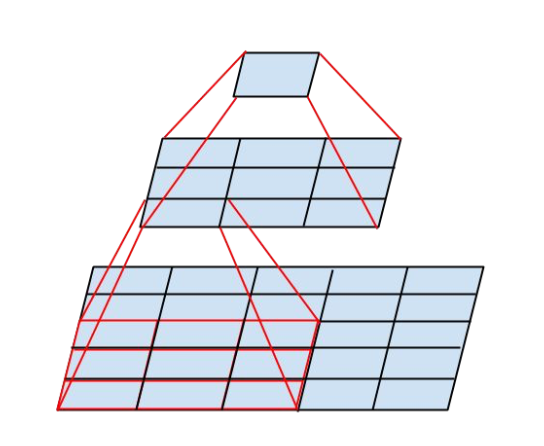
\includegraphics[width=0.6\textwidth]{conv-to-mlp}
  \caption{Una convolución de $5 \times 5$ es un perceptrón multicapa, \emph{per se}.
    (Tomado de \url{https://arxiv.org/pdf/1512.00567.pdf}.)}
  \label{conv-to-mlp}
\end{figure}

La reducción de parámetros por capa CONV implica, además, un entrenamiento más rápido. El costo radica en aplicar\
más convoluciones por cada capa CONV cuyo filtro tiene dimensiones \emph{considerablemente} grandes. Para\
profundizar más en esta idea, imaginemos un filtro de $5 \times 5$. Uno de los beneficios que trae consigo\
el tener un filtro de tamaño ``grande'' (por conveniencia, aquí así lo consideramos) es que la cobertura del\
mismo sobre una imagen le permite capturar mayores detalles de la misma. Ahora, recordemos que una capa CONV\
puede ser vista como un MLP, como se vio en el capítulo anterior; en realidad, ¡el filtro en cuestión\
es una capa totalmente conectada que pasa por toda la imagen de entrada! ¿Por qué no descomponer este MLP\
en varios filtros pequeños aplicados de manera \emph{paralela} sobre la imagen? El resultado es la\
factorización en dos filtros de $3 \times 3$ como se muestra en la Figura \ref{conv-to-mlp}.\par

\begin{figure}[H]
  \centering
  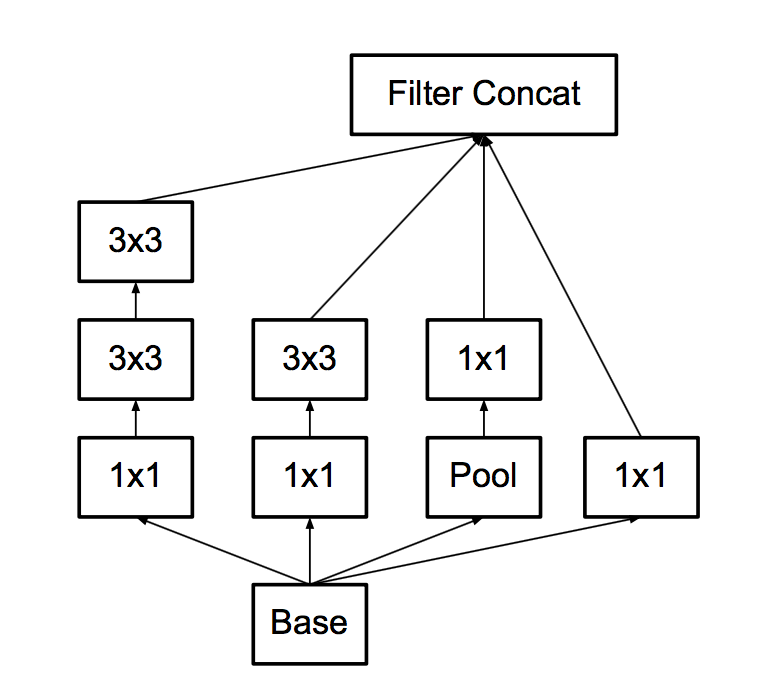
\includegraphics[width=0.6\textwidth]{factorization}
  \caption{Otra manera de factorizar una convolución consiste en paralelizar el cómputo del filtro.
    Cabe destacar que los parámetros de cada nuevo filtro son \emph{compartidos} entre sí,\
    por cada nueva capa. Aquí reemplazamos un filtro de $5 \times 5$ con dos filtros de $3 \times 3$
    y una capa de pooling.
    (Tomado de \url{https://arxiv.org/pdf/1512.00567.pdf}.)}
  \label{factorization}
\end{figure}

En términos propios de la teoría de lenguajes de programación, podemos afirmar que una red neuronal, vista como un\
lenguaje formal, posee una estructura que le permite ser construida de manera \emph{inductiva} a partir\
de pequeñas entidades \emph{bien} definidas. ¿Cómo es que, entonces, se optimiza una red CNN? Minimizando la complejidad\
del cómputo de sus estructuras básicas. En este caso, aprovechamos el cómputo paralelo para factorizar un\
filtro, de donde surgen varios ``hilos de ejecución'' en el grafo de la misma que, deberán ser\
eventualmente \emph{concatenados} en un solo tensor resultante.\par
A la estructura presentada en la Figura \ref{factorization}, se le denomina comúnmente como módulo\
\emph{Inception}. Por otro lado, decimos que una convolución con un filtro de $1 \times 1$ procesa\
\emph{localmente} una imagen de entrada pues realiza una activación (filtrado) exhaustiva a nivel\
de pixeles individuales. En contraste, siguiendo el principio de diseño (\ref{sp-agg}), la reducción\
una adición espacial incorpora dos o más entradas en una. La reducción de dimensiones toma un papel\
clave para garantizar que no haya pérdida de información. No obstante, un incremento en tasa de procesamientos\
locales contra adiciones espaciales favorece la existencia de representaciones dispersas de dimensiones\
altas.

\begin{figure}[H]
  \centering
  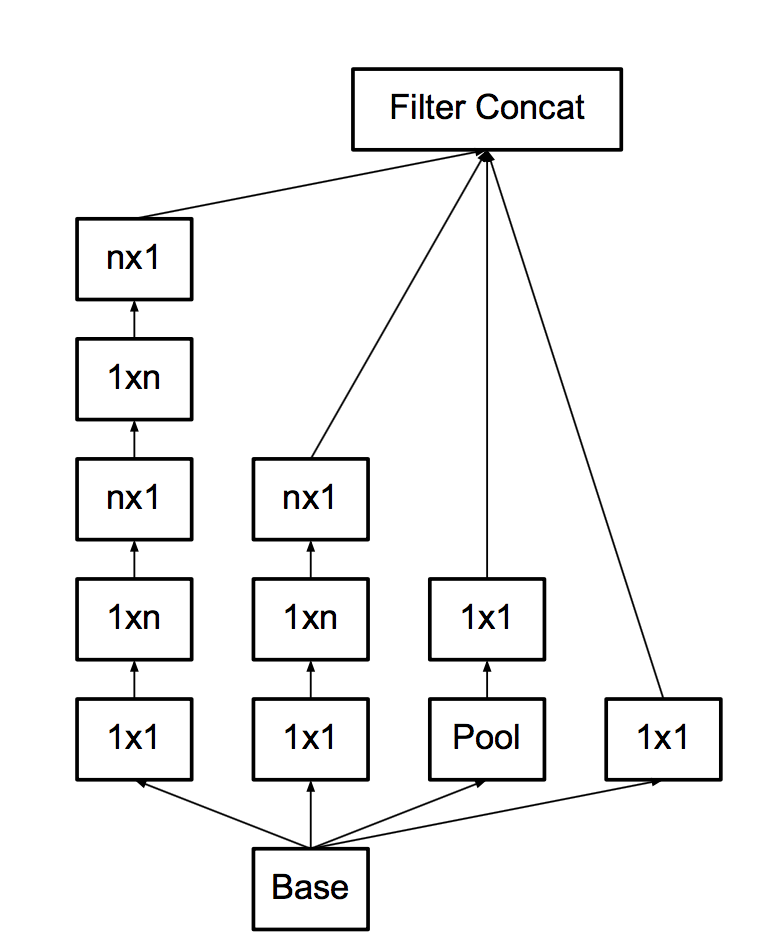
\includegraphics[width=0.6\textwidth]{factorization2}
  \caption{Factorización de una convolución de $n \times n$, donde $n = 7$.
    (Tomado de \url{https://arxiv.org/pdf/1512.00567.pdf}.)}
  \label{factorization2}
\end{figure}

\begin{figure}[H]
  \centering
  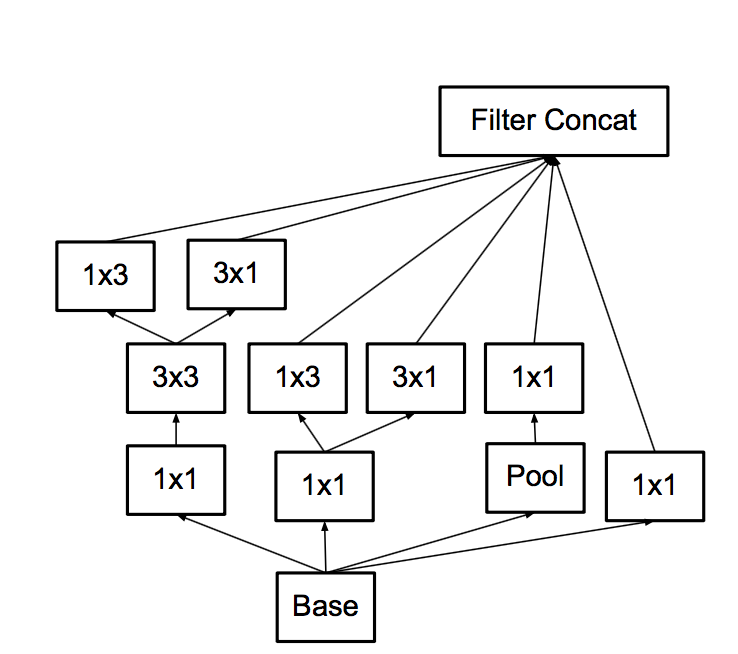
\includegraphics[width=0.6\textwidth]{factorization3}
  \caption{Factorización de una convolución de $8 \times 8$.
    (Tomado de \url{https://arxiv.org/pdf/1512.00567.pdf}.)}
  \label{factorization3}
\end{figure}

Para concluir con esta sección, presentamos las capas que constituyen a la arquitectura Inception\
en la Tabla \ref{capas-inception}.

\noindent
\begin{table}[H]
  \resizebox{\textwidth}{!}{
    \begin{tabular}{|l|c|c|}
      \hline
      \textbf{tipo} & \textbf{tamaño de filtro / zancada} & \textbf{tamaño de la entrada}\\
      \hline \hline
      CONV & $3 \times 3 / 2$ & $299 \times 299 \times 3$ \\
      \hline
      CONV & $3 \times 3 / 1$ & $149 \times 149 \times 32$ \\
      \hline
      CONV con relleno de ceros & $3 \times 3 / 1$ & $147 \times 147 \times 32$ \\
      \hline
      POOL & $3 \times 3 / 2$ & $147 \times 147 \times 64$ \\
      \hline
      CONV & $3 \times 3 / 1$ & $73 \times 73 \times 64$ \\
      \hline
      CONV & $3 \times 3 / 2$ & $71 \times 71 \times 80$ \\
      \hline
      CONV & $3 \times 3 / 1$ & $35 \times 35 \times 192$ \\
      \hline
      $3 \times$ Inception & Figura \ref{factorization} & $35 \times 35 \times 288$ \\
      \hline
      $5 \times$ Inception & Figura \ref{factorization2} & $17 \times 17 \times 768$ \\
      \hline
      $2 \times$ Inception & Figura \ref{factorization3} & $8 \times 8 \times 1280$ \\
      \hline
      POOL & $8 \times 8 / 2$ & $8 \times 8 \times 2048$ \\
      \hline
      LINEAL & logits ($\log$-probabilidades) & $1 \times 1 \times 2048$ \\
      \hline
      MLP-SOFTMAX & clasificador & $1 \times 1 \times 1000$ \\
      \hline
    \end{tabular}
  }
  \caption{
    Las capas que conforman a la arquitectura convolucional \emph{Inception V3}.
    Normalmente, a la dimensión de la última capa se modifica dependiendo de la tarea de clasificación
    deseada. (Tomado de \url{https://arxiv.org/pdf/1512.00567.pdf}.)
  }
  \label{capas-inception}
\end{table}

\section{Poniendo todo junto}

\noindent
Esencialmente, la estructura de cada unidad LSTM usada en la implementación de la RNN es la misma\
que la que fue presentada en la última sección del capítulo anterior. Lo único que cambia es la\
incorporación del tensor de la última capa de Inception ($CNN(I)$), como memoria inicial ($h^{(0)}$).\
Esto se ilustra en la Figura \ref{show_and_tell_architecture}.\par
El entrenamiento de la LSTM se lleva a cabo \emph{desenvolviendo} la recurrencia en un tamaño\
fijo de copias de la LSTM (digamos, $N$). En el tiempo $t+1$, se calcula la probabilidad que tiene\
cada palabra en el diccionario de ser $S_{t+1}$ a partir de $p(S_t|I,S_0,\ldots,S_{t-1})$.\
En resumen,
\begin{align}
  x_{-1} &= CNN(I)\\
  x_t &= W_eS_t,\ \ t \in \{0,\ldots,N-1\}\\
  p_{t+1} &= LSTM(x_t),\ \ t \in \{0,\ldots,N-1\} \label{lstm-output}
\end{align}
donde $x_{-1}$ indica la primera entrada de la LSTM, $x_t$ son las entradas subsecuentes,
$W_e$ es un tensor que incrusta la palabra $S_t$ en el mismo espacio vectorial que $CNN(\cdot)$ y\
$p_{t+1}$ es el tensor de $\log$-probabilidades por cada palabra en el diccionario en el tiempo $t+1$.\
Cabe destacar que $S_t$ se representa matricialmente como un vector codificado \emph{en caliente}
\footnote{
  En una codificación \textbf{en caliente} (\emph{one-hot encoding}, en inglés), se aplica la\
  función indicadora sobre un vector con la dimensión del diccionario de palabras, dejando un 1\
  en el índice que corresponde a la palabra $i$ y 0 en cualquier otro.
}.\par
El error de la arquitectura se calcula mediante la verosimilitud logarítmica negativa,\
sumando cada palabra:
\begin{equation}
  L(I, S) = - \sum_{t=1}^N \log p_t(S_t).
\end{equation}
Acto seguido, se minimiza este error con respecto a todos los parámetros de la LSTM, la última (¡ver la siguiente sección!)\
capa de la CNN y las incrustaciones $W_e$.\par
Finalmente, para la generación de enunciados se utiliza el algoritmo de \textbf{búsqueda por haces}\
(\emph{beam search} en inglés). Iterativamente, se considera el conjunto de las $k$ mejores palabras\
que son candidatas para ser $S_t$ en el tiempo $t$. Esto es una aproximación de
\begin{equation}
  S = \argmax_{S'} p(S'|I)
\end{equation}

\begin{figure}[H]
  \centering
  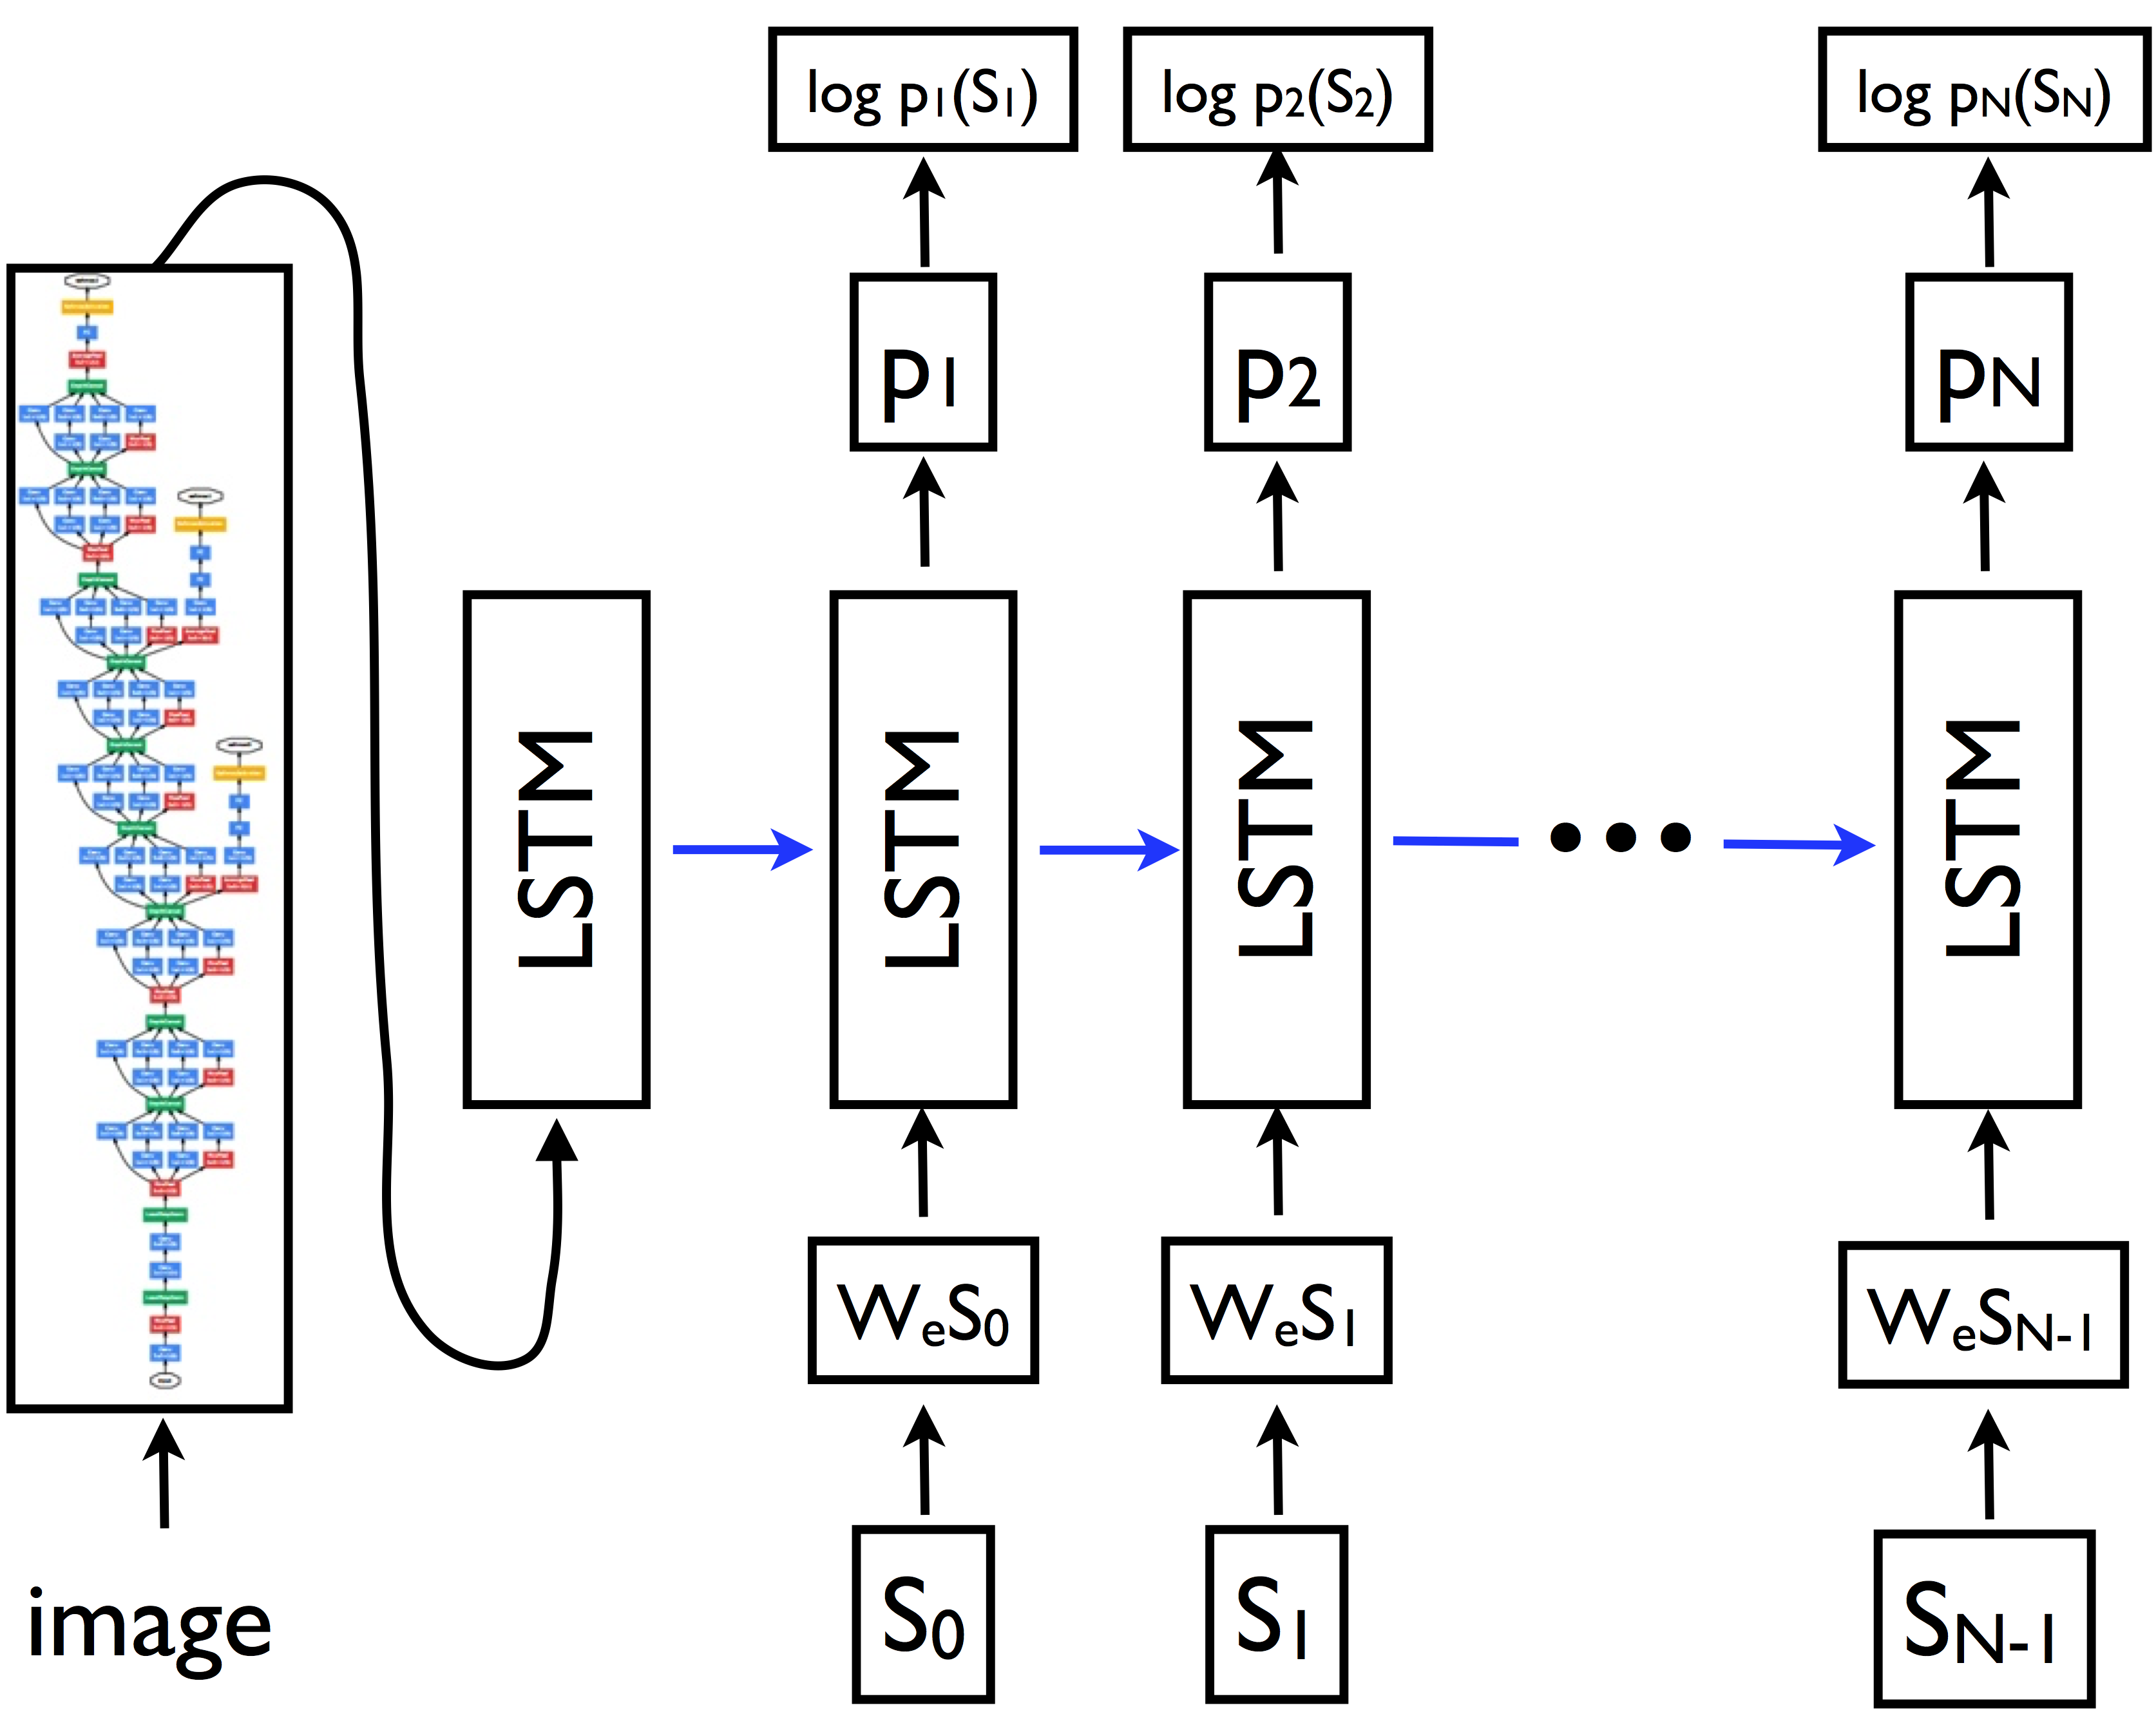
\includegraphics[width=0.9\textwidth]{show_and_tell_architecture}
  \caption{La arquitectura \emph{Show and Tell}, propuesta por Vinyals, \emph{et al},\cite{DBLP:journals/corr/VinyalsTBE14}
    en la cual se conecta una CNN Inception con una LSTM.
    (Tomado de \url{https://arxiv.org/pdf/1411.4555.pdf}.)}
  \label{show_and_tell_architecture}
\end{figure}

\section{Aprendizaje por transferencia}

\noindent
En cada una de las capas de una CNN \emph{profunda}, como las de la Tabla \ref{capas-inception}, se abstraen\
distintas características del conjunto de datos aprendido. ¿Por qué colocar capas MLP tras sucesiones de CONV?\
Otra interpretación de lo que pasa dentro de una capa \emph{densa} consiste en pensar en un cambio de\
espacio vectorial. Cuando la dimensión de la salida es menor que la de la entrada, podemos afirmar que el\
espacio ``objetivo'' comprime la información contenida en las capas previas. Así es como la última\
capa de una arquitectura convolucional preserva la información adquirida tras el entrenamiento.\par
Asumiendo una reducción considerable del error de entropía cruzada y, tras una existosa evaluación\
a través de distintas métricas\footnote{
  Las métricas de evaluación de una CNN se discuten en la Sección \ref{sec:metrics}.
},\
la red convolucional por sí sola pasa a ser un excelente mecanismo de extracción de características de un conjunto\
de datos. Para entrenar una red de la profundidad de \emph{Inception V3} se requiere una cantidad de\
imágenes que muchas veces excede los \verb+10 GB+ en tamaño total. Además, el hecho de reunir semejante tamaño de imágenes\
es, en sí, un tema de gran importancia para las ciencias de datos y un trabajo difícil de lograr.\par
Por ello, la comunidad de \textbf{código abierto} (\emph{open source} en inglés) suele compartir los pesos\
de los parámetros que usaron para entrenar una arquitectura profunda con un conjunto de datos como \emph{Imagenet}.\
Así es como
Dada la riqueza de dicho conjunto de datos, resulta completamente viable suponer que los atributos más importantes\
que comprende un meme de Internet serán identificados por la última capa de \emph{Inception V3}.\par
Consecuentemente, nos ahorramos el entrenamiento de una arquitectura convolucional profunda ``desde cero'' y\
utilizamos los vectores resultantes de un lote de entrenamiento como memoria inicial de la LSTM. Por otro lado,\
el nivel de abstracción que adquiere una CNN entrenada con \emph{Imagenet} es demasiado amplio, en comparación,\
con lo que necesitamos para obtener una buena representación vectorial de un meme\footnote{
  Un meme obtenido de \url{https://memegenerator.net} consiste básicamente en el rostro de un personaje\
  (``viralmente'') famoso centrado en la imagen. Aprender un conjunto de datos obtenido de este sitio se\
  reduce, entonces, a localizar las características más importantes del rostro del personaje en cuestión.
}.\
En este caso, es posible utilizar la distribución probabilística (multivariada) resultante de\
\emph{Inception V3} para mejorar la generalización de una distribución que se enfoque en reconocer atributos de memes.\par
Hablamos, ahora, de un área de estudio conocida como \textbf{aprendizaje por transferencia}.\
A partir del aprendizaje de una distribución $P_1$, ¿qué tanto ésta puede ser explotada para\
aprender otra distribución $P_2$? Para un conjunto de datos como \emph{Imagenet}, es común que las\
primeras capas de un arquitectura profunda se especialicen en detectar pequeños atributos: desde bordes,
cambios de brillo, texturas y partes sombreadas hasta estructuras geométricas básicas (Figura \ref{first-layer}).\
Hace sentido, entonces, utilizar la especialización de estas capas para\
extraer las características más fundamentales de un conjunto de memes.

\begin{figure}[H]
  \centering
  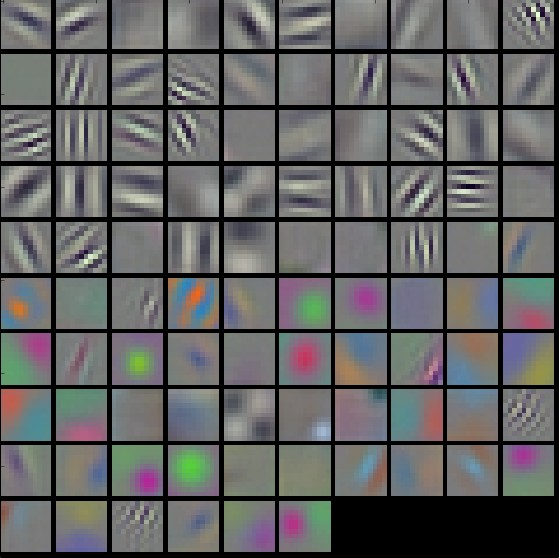
\includegraphics[width=\textwidth]{first-layer}
  \caption{
    Así se ven los filtros entrenados de la primera capa de una CNN profunda.
    En este caso se trata de una AlexNet. La literatura suele conocer a los resultados de estos
    filtros como \emph{``características generales''}.
    (Tomado de \url{http://cs231n.github.io/understanding-cnn/}.)}
  \label{first-layer}
\end{figure}

El procedimiento consecuente a la idea del aprendizaje por transferencia consiste en \textbf{afinar}\
la red neuronal, continuando con el algoritmo de propagación hacia atrás. Esto se hace con un nuevo\
conjunto de datos (el de memes). Usualmente, se propaga el error únicamente sobre algunas de las últimas\
capas (más \emph{específicas}), del modelo; si se vuelven a entrenar todas las capas, cabe la posibilidad\
de llegar a un sobreajuste \cite{DBLP:journals/corr/YosinskiCBL14}.\par
El enfoque tomado para este trabajo consiste en experimentar con una red \emph{Inception V3} como\
extractora de características. Más aún, se probará afinando dicha arquitectura con el conjunto de datos\
reunido. El tamaño del mismo permite hacer dicha afinación.

\section{La arquitectura en acción}\label{sec:arq-accion}

\noindent
Antes de pasar a describir los experimentos realizados para esta tesis, vale la pena echar\
un vistazo formal a cómo funciona el modelo propuesto. De acuerdo a las elecciones de implementación\
(descritas en el siguiente capítulo), la arquitectura tiene tres \verb+modos de operación+:\
\verb+entrenamiento+, \verb+inferencia+ y \verb+evaluación+. Éstos dos últimos consisten en hacer predicciones, utilizando\
el algoritmo de búsqueda por haces para generar un enunciado o añadiendo métricas de evaluación, respectivamente.\par
En cualquiera de estos modos de operación, una entrada del modelo se puede entender como un par ordenado\
$(I, S)$, donde
\begin{itemize}
\item $I$ es un tensor que representa a una imagen (cuadrada) con dimensión fija (\verb+n+), es decir,
  posee tres dimensiones de la forma \verb+[n, n, 3]+;
\item $S$ es un vector cuya dimensión se define por el tamaño del vocabulario obtenido a partir de todas\
  las palabras que conforman el conjunto de datos.
\end{itemize}\par
Usualmente, el vocabulario se construye enumerando todas las palabras existentes (sin repeticiones); $S$ está\
formado, entonces, por los índices numéricos de las respectivas palabras en el vocabulario. En el modo de\
\verb+entrenamiento+, el algoritmo de descenso por el gradiente estocástico sugiere utilizar lotes de\
datos, por lo que los valores de las dimensiones tanto de $I$ como de $S$ suelen ser de la forma\
\verb+[tamaño_lote, n, n, 3]+ y \verb+[tamaño_lote, tamaño_vocabulario]+, respectivamente.\par
En los tres modos, se procede con el cálculo de $CNN(\cdot)$. En el modo de \verb+entrenamiento+\
se sigue hasta el cálculo dado por la Ecuación \ref{lstm-output} y se propaga el error sobre la\
LSTM desenvuelta. Tanto en \verb+inferencia+ como en \verb+evaluación+ se utiliza la LSTM en su\
forma recurrente, dado que será necesario utilizar el tensor resultante de la Ecuación \ref{lstm-output}.
